% Submission to the CoRL 2026 Workshop "Sim-to-Real-to-Field (SRF): The Science of Transfer", Late-Breaking track.
% CoRL 2026 template; 4 pages of main text excluding references; appendices allowed (not reviewed).
\documentclass{article}
\usepackage{corl_2026}
\usepackage{amsmath,amssymb,amsthm}
\usepackage{booktabs}
\usepackage{graphicx}
\usepackage{xcolor}
\usepackage{placeins}
\usepackage{pgfplots}
\pgfplotsset{compat=1.17}
\usepgfplotslibrary{groupplots}
\newtheorem{proposition}{Proposition}
\newcommand{\tbd}[1]{\textcolor{red}{[#1]}}

\title{Let the Fixture Carry Precision in Learned Chains}

\author{Anonymous Author(s)}

\begin{document}
\maketitle

\begin{abstract}
A learned placement policy that is chained compounds its own error, so a transfer gap that doubles the policy's
per-stage error cuts the usable horizon of the chain by about four. We study a classical way to make chain length
insensitive to that gap: after every placement, push the part against a physical reference until contact fixes its
pose. A funnel model makes the trade explicit. Chain failure splits into the policy's error mass beyond the
funnel's capture radius, which is centimetres wide, and the seating residual of the contact step, which is set by
contact physics and fixture geometry, not by the policy. On a simulated Panda line-up with a diffusion policy, four
matched arms show that the gain is contact, not a robot reset or extra motion (restore vs.\ a motion-matched
control, 17:0 discordant chains, $p=1.5\times10^{-5}$). Sweeping the policy-side gap and the
contact model then shows where each transfer factor lands: the restored chain succeeds in 40 of 40 chains across an
$8\times$ range of policy scatter and a 2~cm calibration bias, while unchanged restore code breaks only when fixture
friction rises. That failure is observable on board, from the plate position at which the push stalls.
\end{abstract}

\keywords{sim-to-real transfer, long-horizon manipulation, contact funnels}

\section{Introduction}
Long-horizon manipulation is often built by chaining one learned skill. When later targets are defined relative
to earlier parts, as in assembly, stacking and kitting, a 3~mm error at stage $k$ moves the target of stage $k+1$,
and nothing in the chain pulls the state back. This makes chains unusually fragile under transfer. Every source
of sim-to-real gap that degrades a single placement (camera calibration, lighting, object mass, friction) enters
the chain through the policy's per-stage error $\sigma$, and for a compounding chain the horizon at which half the
chains still succeed scales as $(\tau/\sigma)^2$ for a tolerance $\tau$ (Prop.~\ref{prop:bare}). A policy that is
twice as sloppy in the field as in simulation keeps a quarter of its horizon.

Manipulation has had a remedy for compounding pose error since the 1980s: push the part against something. A
constraining contact maps a whole region of uncertain poses onto one seated pose, which is Mason's
funnel~\citep{mason1985}, preimage backchaining~\citep{lozanoperez1984} and sensorless
orienting~\citep{erdmann1988,goldberg1993}. We ask what such a step does to the \emph{transfer} problem when it
is inserted between the stages of a learned chain, and argue that it changes which quantities have to transfer:
the policy's errors matter only beyond a centimetre-scale capture radius, and the millimetre-scale residual
becomes a property of contact physics and fixture geometry that can be identified and checked on board.

\paragraph{Contributions.}
(1) A funnel model of a chained policy that splits chain failure into a policy term evaluated at the capture
radius and a contact term evaluated at the tolerance (Sec.~\ref{sec:model}). (2) A four-arm protocol, run with a
learned diffusion policy on two task topologies, that separates contact from the robot reset and extra motion any
recovery step also adds (Sec.~\ref{sec:learned}). (3) Transfer sweeps over the policy's scatter and bias, the
and the contact model, which measure each term of the split (Sec.~\ref{sec:transfer}). (4) An
on-board check of the contact term from proprioception alone, and the field tests the model says are needed
(Sec.~\ref{sec:field}).

\paragraph{Related work.} Sim-to-real work usually attacks the policy side of the gap, by randomizing appearance or
dynamics so that $\sigma$ stays small after transfer~\citep{tobin2017,peng2018}, and skill-chaining work regularizes
training so that one skill's terminal states fall inside the next skill's initiation set~\citep{lee2021,scar2024}.
Both change the policy. Classical funnels~\citep{mason1985,lozanoperez1984,erdmann1988,peshkin1988,goldberg1993} and
sequential composition~\citep{burridge1999} change the state instead, and manufacturing models how fixturing stops
variation from propagating through multistage assembly~\citep{jinshi1999,shi2006}; those analyses assume a
mechanics model that certifies capture. BATON~\citep{baton2026} restores the \emph{robot} between learned subtasks with
non-contact motions. We measure what restoring the \emph{part} adds, and what it does to the transfer question.

\section{A Funnel Model of Chain Transfer}
\label{sec:model}
Let $D_k$ be the signed deviation of part $k$ from its nominal pose after stage $k$, with $D_0=0$, and let the
policy land part $k$ with error $\xi_k$ relative to its target, i.i.d.\ with distribution $F_\sigma$ whose scale
$\sigma$ is what transfer degrades. A part succeeds if $|D_k|\le\tau$. In the bare line-up the target is defined by
the predecessor, so $D_k=D_{k-1}+\xi_k$.
\begin{proposition}[bare chains compound]
\label{prop:bare}
If $\xi_k\sim\mathcal{N}(0,\sigma^2)$, the final part succeeds with probability $2\Phi(\tau/\sigma\sqrt N)-1$, an
upper bound on chain success, which falls to one half at $N_{1/2}=(\tau/0.674\,\sigma)^2$. The horizon's elasticity
in the transfer gap is $\partial\log N_{1/2}/\partial\log\sigma=-2$.
\end{proposition}
A contact step behaves differently. Model it as a funnel with capture radius $R$ and seating residual $\eta$: if the
landing deviation $|D_{k-1}+\xi_k|$ (line-up) or $|\xi_k|$ (fixed cells) is at most $R$, the step leaves
$D_k=\eta_k$, an i.i.d.\ draw from the contact step's residual distribution $G$; otherwise the stage is lost.
\begin{proposition}[the funnel splits the transfer burden]
\label{prop:funnel}
If $R>\tau$, the funnel acts at every stage and later stages do not move earlier parts, chain failure is at most
$N\big[\,\Pr_{F_\sigma}(|\xi|>R-\tau)+\Pr_G(|\eta|>\tau)\,\big]$.
\end{proposition}
The first term is the policy's transfer gap, but read at $R-\tau$ rather than at $\tau$, and the second term does not
involve the policy at all. For a Gaussian policy and $R=5\tau$ the first term at $\sigma=\tau$ is $6\times10^{-5}$ per
stage: within the capture radius the horizon's elasticity in $\sigma$ is near zero, and the chain inherits the
transfer properties of the contact step instead ($G$ from friction, stiffness and fixture; $R$ from push geometry).
Two corollaries follow (App.~\ref{app:proofs}): a step that never moves the part, however long, leaves the law of
$(D_1,\dots,D_N)$ unchanged unless it changes the robot state the next placement starts from; and a policy bias $b$
(a calibration offset) is removed entirely while bias plus scatter stays within $R-\tau$.

\section{Setup}
\label{sec:setup}
A Franka Panda in robosuite~\citep{robosuite} (MuJoCo) places 4~cm cubes in a chain of $N$ stages. In the line-up,
stage $k$ targets the actual resting pose of cube $k-1$; in $3\times4$ packing, each cube targets a fixed cell of a
zero-clearance grid. The learned placer is a robomimic diffusion policy~\citep{robomimic,diffusionpolicy} trained by
behavior cloning on 150--300 scripted demonstrations and sampled with 10 DDIM steps. The transfer sweeps use a
scripted placer with injected error, so that $\sigma$, $b$ and the physics can be set exactly. Success means every
cube is within $\tau=8$~mm of its nominal cell at the end of the chain.

\paragraph{Arms.} All arms share seeds and placements. \textit{No reset}: nothing happens between stages.
\textit{Home}: the end effector returns to its pre-placement pose without touching anything, a robot-only reset of the
kind used between VLA subtasks~\citep{baton2026}. \textit{No-op}: home plus a no-contact motion near the part of the
same duration as the restore. \textit{Restore}: the closed gripper, used as a plate, pushes the part against its
references one axis at a time, then homes. Pushes are saturated and stall-terminated, since a proportional
controller's force vanishes exactly where seating needs it; references are found from collision geometry (the
nearest static or seated face in $-x$ and $-y$), so one routine serves both topologies.

\section{Contact, Not Reset or Time}
\label{sec:learned}
\begin{table}[t]
\centering
\caption{Learned diffusion policy, chain success at $\tau=8$~mm (line-up 10 paired seeds, packing 6). In packing
every arm homes the robot. Right: within-stage contraction, the median ratio of a part's deviation after the
post-placement step to its deviation at landing.}
\label{tab:main}
\small
\begin{tabular}{lccccccc}
\toprule
& \multicolumn{3}{c}{3-D line-up} & \multicolumn{3}{c}{$3\times4$ packing} & contraction \\
\cmidrule(lr){2-4}\cmidrule(lr){5-7}
Arm & $N{=}2$ & $N{=}4$ & $N{=}8$ & $N{=}4$ & $N{=}8$ & $N{=}12$ & line-up / pack \\
\midrule
No reset & 0/10 & 0/10 & 0/10 & -- & -- & -- & 1.00 / -- \\
Home     & 7/10 & 0/10 & 0/10 & 0/6 & 0/6 & 0/6 & 1.00 / 1.00 \\
No-op    & 9/10 & 0/10 & 0/10 & 0/6 & 0/6 & 0/6 & 1.00 / 1.00 \\
Restore  & \textbf{10/10} & \textbf{10/10} & \textbf{6/10} & \textbf{6/6} & \textbf{4/6} & 0/6 & \textbf{0.21 / 0.39} \\
\bottomrule
\end{tabular}
\end{table}
Table~\ref{tab:main} gives the learned-policy results. Resetting the robot helps (home vs.\ no reset, 7:0
discordant chains, exact McNemar $p=0.016$), in line with BATON's ablation~\citep{baton2026}, but every non-contact
arm fails all ten line-up chains by $N=4$. Extra motion near the part buys nothing measurable (no-op vs.\ home, 2:0,
$p=0.5$; packing 0:0), as the no-contact corollary predicts. Contact separates the arms: restore beats the
motion-matched control 17:0 on the line-up ($p=1.5\times10^{-5}$) and 16:0 in packing ($p=3\times10^{-5}$). The
mechanism shows per stage: every non-contact arm passes the landing error on unchanged (contraction 1.00), while
restore leaves 0.21 of it on the line-up and 0.39 in packing (bare line-up deviation grows from 3.1 to 155.6~mm over
8 stages; restore stays at 1.2--12.0~mm). Restore costs $2.3\times$ the steps of a bare placement.

\section{Which Side of the Split Does Each Transfer Factor Land On?}
\label{sec:transfer}
\paragraph{Policy-side gap.} We degrade the scripted placer as transfer would: Gaussian scatter $\sigma$ from 2 to
16~mm, and a systematic bias $b$ (a calibration offset) of 5--20~mm at $\sigma=4$~mm, on the $N=8$ line-up with 5
paired seeds per setting. The bare chain fails every chain at every setting, and its worst cube grows with the gap
(median 63~mm at $\sigma=2$~mm, 100~mm at $\sigma=16$~mm, 208~mm at $b=20$~mm). Restore succeeds in 40 of 40 chains at
$\tau=8$~mm across all eight settings, with a median worst cube of 1.8--5.0~mm and a within-stage contraction of
0.07--0.23. The restored chain's error is flat in an $8\times$ range of $\sigma$ and in a bias of half a cube width, as
Prop.~\ref{prop:funnel} predicts inside the capture radius; only the tighter 4~mm tolerance starts to show the gap
(5/5 chains at $\sigma=4$~mm, 1--2/5 at $\sigma\ge12$~mm or $b\ge10$~mm).

\paragraph{Contact-model shift.} The second term of the split belongs to the contact step, so we keep the restore
routine exactly as tuned in robosuite's default physics and execute it under shifted contact models: contact time
constant 0.005--0.04~s, sliding friction $0.5$--$2\times$, pyramidal instead of elliptic friction cones, and
impedance ratio 1 instead of 20 ($N=4$, $\sigma=4$~mm, 2 paired seeds per setting; the run was cut short by memory
on our machine, so these are pilot-scale). Figure~\ref{fig:transfer}b shows the result. Most shifts leave the funnel
intact (median worst cube 0.1--2.8~mm, all chains successful). Friction does not: at $1.5\times$ and $2\times$ the
contraction rises to 0.67 and 0.99, so the step stops removing error, and the worst cube reaches 11.7 and 13.6~mm.
Very stiff contact costs less (5.8~mm); the bare chain fails everywhere. The burden has moved, not vanished: to
the fixture's friction, which a field team can measure with a pull test.

\begin{figure}[t]
\centering
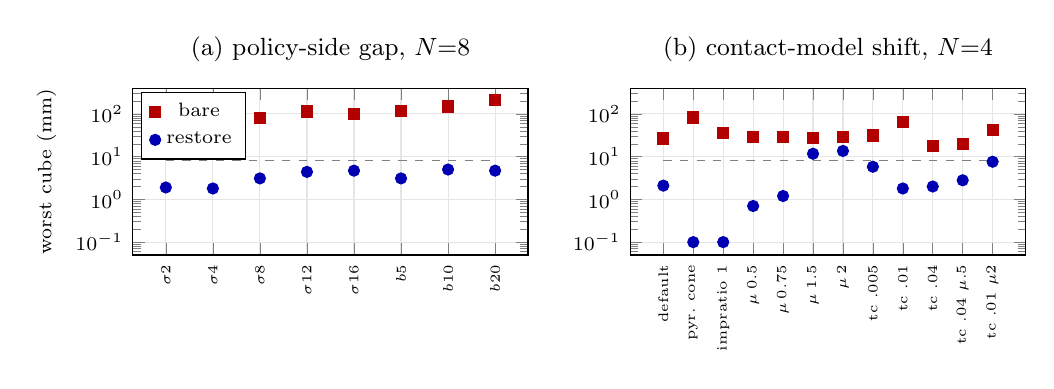
\begin{tikzpicture}
\begin{groupplot}[group style={group size=2 by 1, horizontal sep=1.3cm},
  width=6.6cm, height=3.7cm, ymode=log, ymin=0.05, ymax=400,
  ylabel={worst cube (mm)}, ylabel style={font=\scriptsize}, tick label style={font=\scriptsize},
  title style={font=\small}, xticklabel style={rotate=90, anchor=east, font=\tiny},
  grid=major, grid style={draw=gray!20}, legend style={font=\scriptsize, at={(0.02,0.98)}, anchor=north west}]
\nextgroupplot[title={(a) policy-side gap, $N{=}8$}, symbolic x coords={s2,s4,s8,s12,s16,b5,b10,b20},
  xtick=data, xticklabels={$\sigma$2,$\sigma$4,$\sigma$8,$\sigma$12,$\sigma$16,$b$5,$b$10,$b$20}]
\addplot[only marks, mark=square*, color=red!70!black] coordinates
  {(s2,62.7)(s4,53.6)(s8,79.7)(s12,114.0)(s16,99.5)(b5,117.0)(b10,149.0)(b20,207.5)};
\addlegendentry{bare}
\addplot[only marks, mark=*, color=blue!70!black] coordinates
  {(s2,1.9)(s4,1.8)(s8,3.1)(s12,4.4)(s16,4.7)(b5,3.1)(b10,5.0)(b20,4.7)};
\addlegendentry{restore}
\addplot[dashed, gray, domain=0:8, forget plot] coordinates {(s2,8)(b20,8)};
\nextgroupplot[title={(b) contact-model shift, $N{=}4$}, ylabel={},
  symbolic x coords={def,cone,imp,m05,m075,m15,m20,t005,t01,t04,t04m05,t01m20}, xtick=data,
  xticklabels={default,pyr.\ cone,impratio 1,$\mu\,0.5$,$\mu\,0.75$,$\mu\,1.5$,$\mu\,2$,tc .005,tc .01,tc .04,tc .04 $\mu$.5,tc .01 $\mu$2}]
\addplot[only marks, mark=square*, color=red!70!black] coordinates
  {(def,26.7)(cone,82.2)(imp,35.8)(m05,28.4)(m075,29.2)(m15,27.2)(m20,28.6)(t005,31.2)(t01,64.7)(t04,17.4)(t04m05,19.7)(t01m20,41.6)};
\addplot[only marks, mark=*, color=blue!70!black] coordinates
  {(def,2.1)(cone,0.1)(imp,0.1)(m05,0.7)(m075,1.2)(m15,11.7)(m20,13.6)(t005,5.8)(t01,1.8)(t04,2.0)(t04m05,2.8)(t01m20,7.6)};
\addplot[dashed, gray, forget plot] coordinates {(def,8)(t01m20,8)};
\end{groupplot}
\end{tikzpicture}
\caption{Median worst-cube deviation per setting (log scale; dashed line: $\tau=8$~mm). (a) Degrading the placer
(scatter $\sigma$ and bias $b$, mm) moves the bare chain but not the restored one. (b) Executing the unchanged
restore under shifted contact physics: only high friction and very stiff contact move it toward the tolerance.}
\label{fig:transfer}
\end{figure}

\paragraph{On-board seat check.} The contact term can also be observed at deployment. Where the plate stalls at the
end of the final push, read from proprioception and corrected by one offset calibrated in default physics, estimates
the seated part's deviation to a median of 0.3--1.7~mm (90th percentile 1.0--4.2~mm) over 260 restore stages of the
gap sweep, abstaining when the part was already seated and the plate never reached it. Under the shifted contact
models, where the offset was not recalibrated, the error grows to 0.3--4.8~mm, and flagging a stage when the estimate
exceeds $\tau$ catches 7 of the 11 stages that actually ended outside tolerance, with 5 false alarms in 64 stages. The failure friction introduces, a push arrested short of
its fence, is one the arm can feel.

\section{Toward the Field}
\label{sec:field}
Read as a recipe for transfer, the split says what to validate on hardware and what to stop worrying about.
\textit{Measure the funnel, not the policy:} the capture radius $R$ (here at least 2~cm, since biases of 20~mm and
scatter of 16~mm were absorbed) and the seating residual $G$ on the real fixture, which needs only scripted pushes of
deliberately misplaced parts, no learned policy. \textit{Identify friction first:} it is the one contact parameter
in our sweep that broke the funnel, and the one most likely to differ between a simulated and a real fixture
(surface finish, dust, wear). \textit{Monitor the stall:} a plate that stops short of where the fixture says it
should is an on-board flag of a failed seat, and the place to trigger a retry. \textit{Spend randomization on the
policy only up to $R$:} once its errors are inside the capture radius, further policy-side robustness buys no chain
length.

\paragraph{Limitations.} Every number is from MuJoCo, with cubes only; we have not measured $R$ or $G$ on hardware.
The contact sweep is pilot-scale (2 seeds per setting). The restore routine reads part poses from the simulator to
plan its approach, so perception error enters only through that approach. In zero-clearance packing, late pushes
shift the finished block by 2--35~mm, so restore fails all chains at $N=12$: the model's assumption that stages do
not disturb each other is where it breaks.
\paragraph{Conclusion.} Contact re-seating lets the policy be centimetre-accurate and takes the millimetres from
the fixture; the next step is measuring a real fixture's capture radius and seating residual.

\bibliography{refs}

\appendix
\section{Proofs}
\label{app:proofs}
\textit{Proposition~\ref{prop:bare}.} Unrolling $D_k=D_{k-1}+\xi_k$ from $D_0=0$ gives $D_N=\sum_{k\le N}\xi_k\sim
\mathcal{N}(0,N\sigma^2)$, so $\Pr(|D_N|\le\tau)=2\Phi(\tau/\sigma\sqrt N)-1$. Chain success requires the final part to
succeed, which bounds it above. Since $2\Phi(x)-1=\tfrac12$ at $x\approx0.674$, the bound is one half at
$N_{1/2}=(\tau/0.674\sigma)^2$, and $\log N_{1/2}=2\log\tau-2\log(0.674\sigma)$ has derivative $-2$ in $\log\sigma$.

\textit{Proposition~\ref{prop:funnel}.} Let $A_k=\{|\xi_k|>R-\tau\}$ and $B_k=\{|\eta_k|>\tau\}$. On the complement of
$\bigcup_k(A_k\cup B_k)$ every part succeeds, by induction on $k$: if $|D_{k-1}|\le\tau$ (true for $D_0=0$), the
landing deviation is at most $|D_{k-1}|+|\xi_k|\le\tau+(R-\tau)=R$ (and $|\xi_k|\le R$ when targets are fixed cells),
so the funnel captures the part and leaves $D_k=\eta_k$ with $|\eta_k|\le\tau$. The model assumes later stages do
not move earlier parts, so the final configuration is the per-stage one. A union bound over the $2N$ events gives
failure at most $N[\Pr(|\xi|>R-\tau)+\Pr(|\eta|>\tau)]$. For $\xi\sim\mathcal{N}(0,\sigma^2)$, $R=5\tau$ and
$\sigma=\tau$, $\Pr(|\xi|>4\tau)=2(1-\Phi(4))\approx6.3\times10^{-5}$.

\textit{No-contact corollary.} If the post-placement step is the identity on part poses, $D_k$ is the same function of
$(\xi_1,\dots,\xi_k)$ as in the bare chain; if in addition the step leaves the law of the next $\xi$ unchanged, the joint
law of $(D_1,\dots,D_N)$ is unchanged. A no-contact step can therefore act only through the robot state the next
placement starts from, which is what home vs.\ no reset measures.

\textit{Bias corollary.} Replace $\xi_k$ by $b+\xi_k$ in the proof of Proposition~\ref{prop:funnel}: the induction goes
through whenever $|b+\xi_k|\le R-\tau$, and $D_k=\eta_k$ does not depend on $b$, so the bias is removed and the
policy term becomes $\Pr(|b+\xi|>R-\tau)$.

\textit{Linear contraction.} The measured contraction ratio fits a weaker, linear version of the funnel,
$D_k=aD_{k-1}+c\,\xi_k$ with inheritance $a$ and contraction $c$. For $|a|<1$ and Gaussian $\xi$,
$\mathrm{Var}(D_k)=c^2\sigma^2(1-a^{2k})/(1-a^2)\le c^2\sigma^2/(1-a^2)$ for every $k$, so the error is bounded at every
horizon, but still proportional to $\sigma$; the funnel model above is the limit in which the residual stops
depending on the landing error, which is what the transfer sweeps test.

\end{document}
